I have implemented alignments in the \mmt system.  Moreover, I have
created a public repository~\cite{Alignments:on} and seeded it with a number of alignments
(currently $\approx12000$) including the ones mentioned above and below in \autoref{sec:crosslib:alignments:manually}, the README of this
repository furthermore describes the syntax for alignments above as well as the URI
schemata for several proof assistants.  The \mmt system can be used to parse and serve all
these alignments, implement the transitive closure, and (if possible) translate
expressions according to alignments (see \autoref{sec:crosslib:translate} for the details). Available alignments are shown in the \mmt browser.

\paragraph{} As an example service, I built a prototypical alignment-based math dictionary collecting formal and informal resources.\footnote{Unfortunately, due to recent changes in the \mmt API, the original dictionary is no longer compatible with the current code base and needs to be reimplemented at some point in the future.}
For this we extend the above grammar by the following:
\begin{center}
\begin{tabular}{l@{\tb}c@{\tb}l}
	Alignment & \bbc & String URI $\rep{\bnfbracket{\mathrm{String} = "\mathrm{String}"}}$
\end{tabular}
\end{center}
This assigns a mathematical concept (identified by the string) to a formal or informal resource (identified by the URI). The dictionary uses the above public re\-po\-si\-tory, so additions to the latter will be added to the former. We have imported the $\approx$~50,000 conceptual alignments from~\cite{GinCor:nnexus:14}, although we chose not to add them to the dictionary yet, since the majority of them are (due to the different intention behind the conceptual mappings in Nnexus) dubious, highly contextual or otherwise undesirable.

Each entry in the dictionary shows snippets from select online resources if available
(\autoref{fig:aligns1}), lists the associated formal statements (\autoref{fig:aligns2})
and available alignments between them (\autoref{fig:aligns3}), and allows for
conveniently adding new individual URIs to concept entries as well as new formal
alignments (Figures \ref{fig:aligns1} and \ref{fig:aligns4} respectively).
%\footnote{A
%  well-seeded example are the entries for cartesian products at \cpmathhuburl{} and the
%  connected entry for product types}

\begin{figure*}[ht!]\centering
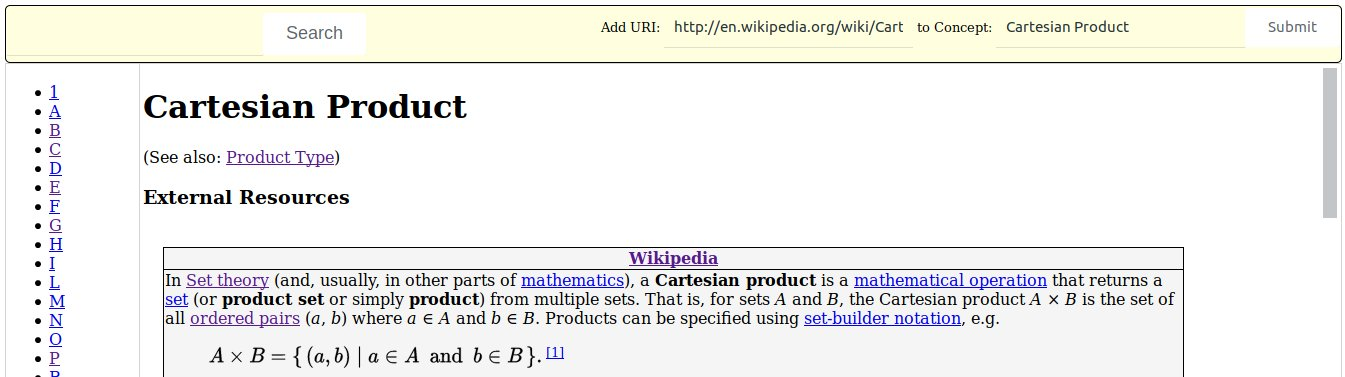
\includegraphics[width=\textwidth]{img/align-mathhub1.jpg}
\caption{The Alignment-based Dictionary --- External Resources}\label{fig:aligns1}
\end{figure*}
\begin{figure*}[ht!]\centering
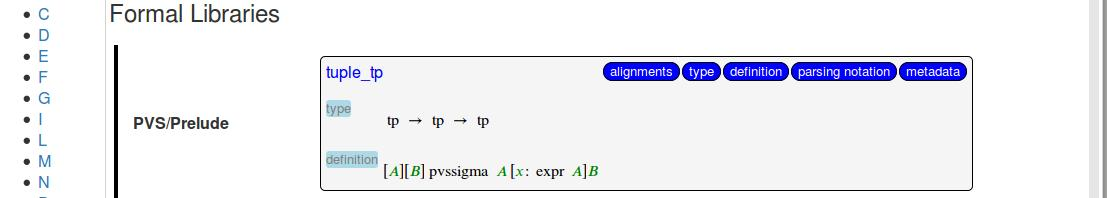
\includegraphics[width=\textwidth]{img/align-mathhub2.jpg}
\caption{The Alignment-based Dictionary --- Formal Resources}\label{fig:aligns2}
\end{figure*}

\begin{figure*}[t!]\centering
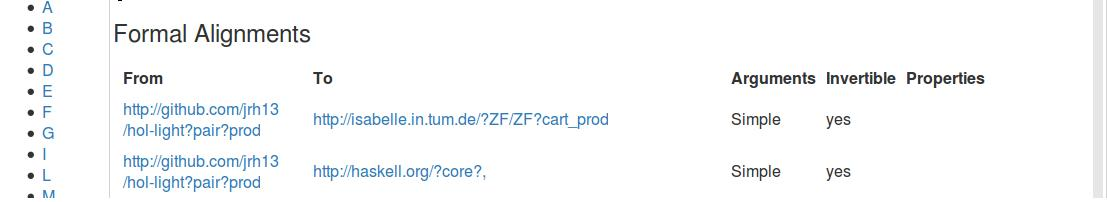
\includegraphics[width=\textwidth]{img/align-mathhub3.jpg}
\caption{The Alignment-based Dictionary --- Available Alignments}\label{fig:aligns3}
\end{figure*}
\begin{figure*}[t!]\centering
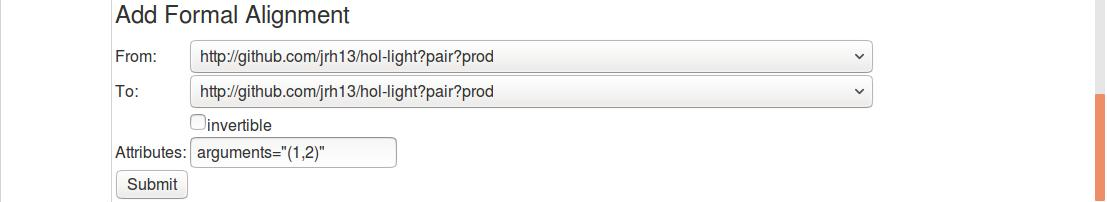
\includegraphics[width=\textwidth]{img/align-mathhub4.jpg}
\caption{The Alignment based Dictionary - Field for Adding Alignments}\label{fig:aligns4}
\end{figure*}

%\begin{figure}
%
\includegraphics[width=\textwidth]{formals.jpg}
%\caption{The MMT Server showing formal alignments with content-aware right-click menu}\label{fig:formals}
%\end{figure}

%%% Local Variables:
%%% mode: latex
%%% TeX-master: "paper-cicm2"
%%% End:

%  LocalWords:  centering includegraphics textwidth emph emph emph
